V~této kapitole je popsána implementace generátoru syntetických datových sad vytvořeného v~rámci této práce. Dále je zde popsán proces vytváření detektoru dopravních značek, jeho trénovaní, vyhodnocení a~iterativního zlepšování úspěšnosti.


%%%%%%%%%%%%%%%%%%%%%%%%%%%%%%%%%%%%%%%%%%%%%%%%%%%%%%%%%%%%%%%%%%%%%%%%%%%%%%%%%%%%%%%%%%%


\section{Generátor syntetických datových sad}
\label{syntDataset}
Generování syntetických datových sad pro trénování hlubokých neuronových sítí se stává čím dál populárnější technikou, která usnadňuje proces trénovaní o~nutnost anotovat datovou sadu (či rozšíření existující datové sady) a~zároveň umožňuje dosažení dobré úspěšnosti detekce/klasifikace. Avšak problém je dokázat generovat datovou sadu tak, aby model na ní trénovaný dokázal správně generalizovat na reálných snímcích, což je čím dál častěji předmětem výzkumu a~bude popsáno i~v~této práci.

Pro generování se nabízí hned několik způsobů. Aplikační rámce jako např. PyTorch či TensorFlow obsahují zabudované \uv{generátory}, které lze využít pro rozšíření již existující datové sady. Ty fungují na principu modifikace jednotlivých snímků datové sady (např. otočení snímku kolem osy \emph{y}, změna světelných podmínek, apod.) a~jejich následné připojení k~datové sadě. Další způsob využívaný zejména pro komplexní objekty, jako je například tvář člověka, je vymodelování objektu (např. v~programu \emph{Blender}) a~poté pomocí skriptu \uv{nafocení} tohoto objektu z~různých uhlů a~za různých světelných podmínek. Pro generování plných snímků, které jsou pro trénování neuronové sítě YOLO potřeba, lze využít techniku umisťování těchto objektů do snímků pozadí a~modifikaci jejich vzhledu za účelem dosažení větší variability vzniklé datové sady. Poslední zmíněnou technikou je GAN\footnotemark. Tato technika, jak již jméno napovídá, je založena na \uv{zápasení} dvou neuronových sítí a~slouží mimo jiné pro generování syntetických snímků. Je to ovšem metoda učení bez učitele, a~proto se nedá použít pro generování objektů do plných snímků.

\footnotetext{GAN -- \emph{Generative adversarial network}.}

Systém YOLO je trénovaný na plných snímcích, a~proto jak bylo navrženo, byl v~této práci využit způsob umisťování dopravních značek do plných snímků pozadí. Dále byla získána sada snímků z~palubní kamery a~veškeré snímky obsahující dopravní značky byly odstraněny, protože by negativně ovlivňovaly proces trénovaní.

\subsection*{Efekty aplikované na značky}
\label{syntDatasetEfekty}
Aby bylo dosaženo větší variability datové sady a~konvoluční neuronová síť se byla schopna naučit co nejvíce vlastností dopravních značek, bylo před samotným vložením značky do pozadí provedeno několik operací upravující vzhled značky. Seznam operací, které se s~určitou pravděpodobností aplikují na vyřezané dopravní značky, je následující:

\begin{itemize}
    \item \textbf{Gamma korekce} -- Slouží k~simulaci různých světelných podmínek. Pravděpodobnost aplikace tohoto efektu je $15\,\%$.
    \item \textbf{Úprava jasu} -- Slouží k~simulaci různých světelných podmínek. Pravděpodobnost aplikace tohoto efektu je $15\,\%$.
    \item \textbf{Úprava jasu podle pozadí} -- Slouží k~získání průměrného osvětlení v~místě, kam bude dopravní značka umístěna a~následné úpravě jasu značky podle získané hodnoty. Lze nahradit za předchozí efekt.
    \item \textbf{\emph{Salt and pepper} šum} -- Slouží k~simulaci poškození značky. Pravděpodobnost aplikace tohoto efektu je $5\,\%$.
    \item \textbf{Gaussovský šum} -- Slouží k~simulaci poškození značky. Pravděpodobnost aplikace tohoto efektu je $5\,\%$.
    \item \textbf{Překrytí části značky} -- Simuluje běžně se vyskytující překrytí značky. Pravděpodobnost aplikace tohoto efektu je $5\,\%$.
    \item \textbf{Gradient osvětlení} -- Simuluje reálné osvětlení značek. Pravděpodobnost aplikace tohoto efektu je $15\,\%$.
    \item \textbf{Rotace v~ose Z} -- Simuluje záběr z~různých úhlů. Pravděpodobnost aplikace tohoto efektu je $25\,\%$.
    \item \textbf{Rotace v~ose Y} -- Simuluje záběr z~různých úhlů. Pravděpodobnost aplikace tohoto efektu je $25\,\%$.
    \item \textbf{Rozmanání značky} -- Simuluje vyšší rychlost vozidla či nižší kvalitu kamery. Pravděpodobnost aplikace tohoto efektu je $5\,\%$.
    \item \textbf{Úprava barvy (HSV)} -- Simuluje značky různých Evropských norem (viz obrázek~\ref{kolazStopky}). Pravděpodobnost aplikace tohoto efektu je $10\,\%$.
    \item \textbf{Změna velikosti značky} -- Simuluje různé vzdálenosti značky od kamery. Pravděpodobnost aplikace tohoto efektu je $90\,\%$.
\end{itemize}

Naopak techniky, které úspěšnost nezvýšily, či dokonce snížily jsou následující:

\begin{itemize}
    \item Rotace značky kolem osy \emph{y}
    \item Přidání luminiscenčního podkladu značek
    \item Přidání ocelové konstrukce značek
    \item Výběr pozic, kam značku umístit a~následná úprava velikosti podle umístění
\end{itemize}

Z~důvodu, že se dopravní značky nachází většinou po stranách silnice, bylo provedeno několik pokusů s~umisťováním značek pouze na okraje, a~to tak že čím blíže byly středu, tím menší velikosti nabývaly (simulace reálného prostředí). Tyto pokusy však neprokázaly zvýšení úspěšnosti. Luminiscenční podklad i~ocelová konstrukce měly za úkol přidat přirozený kontext, ve kterém se značky nachází. Tyto přidané objekty ovšem výrazně snižovaly úspěšnost detekce. Jedna z~vlastností mnoha značek je, že jsou osově souměrné, a~proto byla vyzkoušena také rotace značek kolem osy \emph{y} (kromě značek obsahující šipky vlevo/vpravo apod.), ale ke zlepšení úspěšnosti to nevedlo.

\subsection*{Způsob generování s~transparentními značkami}
\label{syntDatasetTransparent}
Tato technika je založena na principu umisťování transparentních značek (obsahující alfa-kanál) do snímků pozadí. Výhodou tohoto přístupu je, že kolem značky nevzniká výrazná přestupná hrana, jako je tomu u~druhého způsobu používající vyřezané značky.

\begin{figure}[H]
    \centering
    \tmpframe{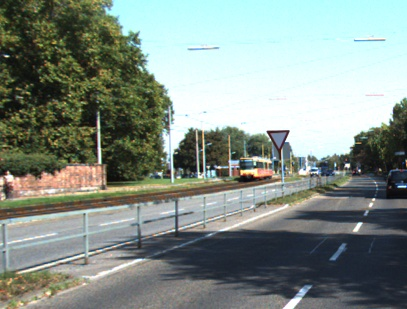
\includegraphics[width=0.495\linewidth]{figures/implementace/giveway_transparent.png}}\hfill
    \tmpframe{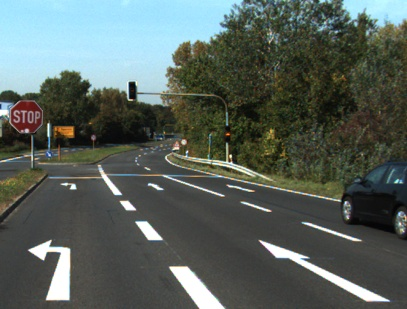
\includegraphics[width=0.495\linewidth]{figures/implementace/stop_transparent.png}}\\
    \tmpframe{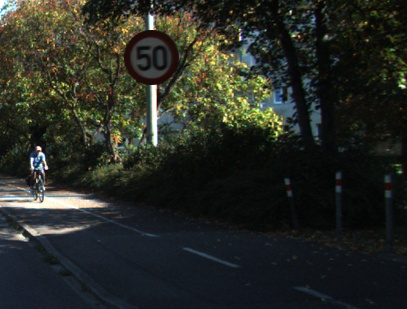
\includegraphics[width=0.495\linewidth]{figures/implementace/synt_50.png}}\hfill
    \tmpframe{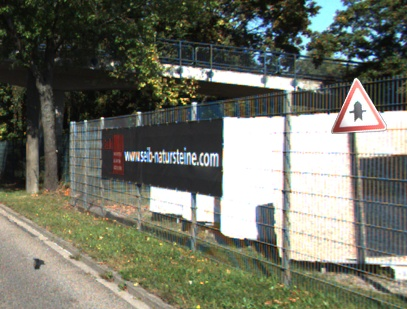
\includegraphics[width=0.495\linewidth]{figures/implementace/synt_junction.png}}
    \caption{Příklad vygenerovaných dat za pomoci transparentních značek. Značkám bylo před vložením do snímku pozadí upraveno osvětlení, velikost a~natočení.}
    \label{fig:datasetCropped}
\end{figure}

Naopak nevýhodou tohoto přístupu je, že aby bylo dosaženo jisté variability takto vygenerované datové sady, bylo by potřeba velké množství značek vyřezaných z~reálných snímků. Tento problém se dá řešit pomocí již zmíněných efektů aplikovaných na dopravní značky popsaných v~sekci \ref{syntDatasetEfekty} a~vizualizovaných na obrázku \ref{fig:stopImplementace}.

\begin{figure}[H]
    \centering
    \tmpframe{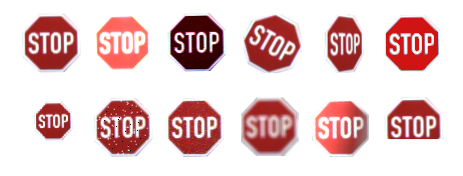
\includegraphics[width=0.99\linewidth]{figures/implementace/znacky.png}}
    \caption{Příklad aplikace všech efektů modifikujících vzhled dopravních značek na jedné značce typu \emph{stop}. Originál vlevo nahoře.}
    \label{fig:stopImplementace}
\end{figure}

Pravděpodobnost aplikace efektu je dána pravděpodobností s~rovnoměrných rozložením, takže se běžně stává, že se aplikuje více efektů na jednu značku (například natočení, změna jasu i~přidání šumu). Každý efekt používá jiné hodnoty, například natočení značky se udává ve stupních. Z~daného, předem definovaného, rozsahu aplikovaných hodnot se pseudonáhodně vybere hodnota při každé aplikaci efektu. Kdyby se při každé aplikaci efektu používaly stejné hodnoty, vzhled značek by se začal brzy opakovat.

Pravděpodobnost aplikace efektu i~rozsah aplikovaných hodnot byly pečlivě vybírány a~upravovány jak pomocí experimentů, tak inspirací vzhledu značek z reálného světa. Například vizuálně poškozené značky se příliš často nevyskytují, proto byla pro přidání šumu zvolena poměrně nízká pravděpodobnost. Naopak různé světelné podmínky či natočení značek jsou běžně se vyskytující jevy, proto jim byla přiřazena poměrně vysoká pravděpodobnost aplikace.

Při implementaci jednotlivých efektů byla vždy prováděna kontrola realističnosti vzhledu vygenerovaných značek. Tzn. zda vygenerované značky vypadají jako by pocházely z~reálného světa. Dosažení opravdu reálného vzhledu je velmi problematické a~vyžadovalo by složitou 3D analýzu jak značky, tak pozadí, kam se značka umisťuje. Ani při dosažení realistického vzhledu (pro člověka) není jisté, zda se dokáže neuronová síť naučit potřebné vlastnosti a~dokáže poté správně generalizovat na reálných snímcích. Lidské oko je totiž více citlivé na jiné faktory, než počítač.

\subsection*{Způsob generování s~ořezanými značkami}
\label{syntDatasetOrezane}
Tento způsob je založen na použití reálných snímků vyřezaných dopravních značek určených pro trénování klasifikátorů. Těchto značek je velké množství, ale nevýhodou je, že po vložení do snímku pozadí kolem těchto značek vzniká výrazná přestupná hrana, jak lze vidět na obrázku \ref{fig:datasetCropped} (vlevo), která negativně ovlivňuje proces trénování. Řešením je použití tzv. \emph{Poisson blending}, které kombinuje gradienty a~intenzity barev obou obrázků a~ve výsledku to vypadá tak, že objekt do daného kontextu patří. Nevýhodou je, že algoritmus \emph{Poisson blending} začíná počítat pouze od hraničních bodů, kam se objekt umisťuje, a~proto pokud jsou tyto hraniční body příliš světlé, sníží se i~intenzita barev vkládané značky a~ve výsledku není téměř vidět. Podobně tomu je pokud jsou hraniční body příliš tmavé, až černé \cite{poissonEditing}. Příklad výsledku vložení pomocí techniky \emph{Poisson blending} lze vidět na obrázku \ref{fig:datasetCropped} (vpravo). Použité vyřezané značky pochází z~Německé datové sady, protože použití značek vyřezaných z~Belgické datové sady, na které se později provádělo vyhodnocení by mohlo zkreslit výsledky.

\begin{figure}[H]
    \centering
    \tmpframe{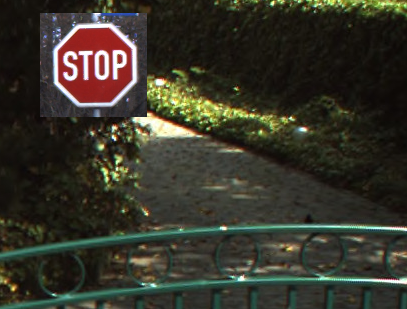
\includegraphics[width=0.49\linewidth]{figures/implementace/stop_cropped.png}}\hfill
    \tmpframe{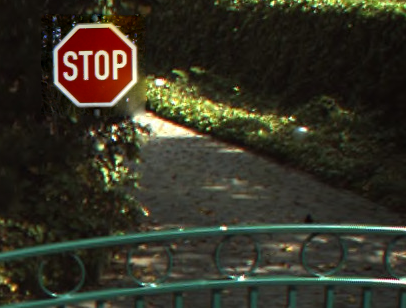
\includegraphics[width=0.49\linewidth]{figures/implementace/stop_poisson.png}}
    \caption{Porovnání vložení ořezané dopravní značky do pozadí bez použití (\textbf{vlevo}) a~s~použitím (\textbf{vpravo}) techniky \emph{Poisson blending}.}
    \label{fig:datasetCropped}
\end{figure}


\subsection*{Množství generovaných dat}
Pro trénování na syntetických datech bylo potřeba zjistit optimální počet generovaných značek na třídu. V~tabulce \ref{tab:pocetSnimkuUspesnost} lze vidět závislost počtu syntetických snímků na výsledné úspěšnosti. Jak lze z~tabulky vyčíst, mezi $200$, $500$ a~$1000$ snímky se vyskytují velké skoky v~úspěšnosti, zatímco mezi $1000$ a~$2000$ se úspěšnost již téměř nezvýšila, zato se razantně prodloužila doba trénování. Jako optimální počet pro budoucí trénování na syntetických datech tedy vyšlo $1000$ značek na třídu.

\begin{table}[h]
	\vskip6pt
	\caption{Závislost úspěšnosti YOLOv3-608 na množství syntetických snímků na třídu.}
	\centering
	\begin{tabular}{cc}
		\toprule
		Počet snímků & Úspěšnost v~mAP\\
		\midrule
		$200$  & $63.2\,\%$ \\
		$500$  & $77.9\,\%$ \\
		$\textbf{1000}$ & $86.3\,\%$ \\
		$2000$ & $\textbf{87.6}\,\%$ \\
		\bottomrule
	\end{tabular}
	\label{tab:pocetSnimkuUspesnost}
\end{table}

%%%%%%%%%%%%%%%%%%%%%%%%%%%%%%%%%%%%%%%%%%%%%%%%%%%%%%%%%%%%%%%%%%%%%%%%%%%%%%%%%%%%%%%%%%%

\section{Konfigurace neuronové sítě při trénovaní a~testování}
\label{cnnKonfigurace}
Pro konfiguraci neuronové sítě se používá konfigurační soubor, \texttt{yolo-train.cfg}, při jehož studiu a~popisu jsem vycházel z~\cite{darknet_config, darknet_anchors}. Nejdůležitější parametry, které lze v~rámci konfiguračního souboru nastavit a~se kterými bylo v~rámci této práce experimentováno jsou následující:

\begin{itemize}
    \item \textbf{anchors} -- Výstupní hodnoty neuronové sítě YOLO neudávají přímo výšku a~šířku ohraničujícího boxu, ale udávají pouze \emph{offset} vůči před-definovaným \uv{kotvám} (anglicky \textbf{\emph{anchors}}) s~nejvhodnější velikostí. Tyto kotvy se vyskytují ve vrstvách \texttt{[yolo]} a~jsou definovány následovně: \texttt{anchors = 4,7, 7,15, 13,25,   25,42, 41,67,\\ 75,94, 91,162, 158,205, 250,332}.
    \item \textbf{mask} -- Každá \texttt{[yolo]} vrstva potřebuje vědět o~všech kotvách, ale jen některé z~nich může použít. Proto se do těchto vrstev zavedl seznam \emph{mask}, ve kterém se udají indexy kotev, které smí daná vrstva použít. Pro použití pouze prvních třech kotev lze použít \texttt{mask = 0,1,2}.
    \item \textbf{filters} -- Udává počet konvolučních jader v~dané vrstvě. Nejvhodnější počet filtrů je podle autorů \texttt{filters = (num\_classes + 5) * 3}. Hodnota 5 označuje počet predikovaných hodnot pro jeden ohraničující box (x, y, výška, šířka a~skóre \emph{objectness}) a~3 v~tomto případě označuje počet kotev.
    \item \textbf{activation} -- Určuje aktivační funkci vrstvy. Může být např. \emph{ReLu}, \emph{sigmoid}, \emph{tanh}, \emph{linear}, \emph{leaky}, apod.
    \item \textbf{random} -- Pokud se rovná jedné, daná vrstva mění velikost vstupního snímku vždy po několika dávkách na různé velikosti.
    \item \textbf{angle} -- Otočení vstupního snímku o~uvedený počet stupňů.
    \item \textbf{batch} -- Dávka, tedy množství snímků k~dopředné propagaci skrze neuronovou síť sloužící k~výpočtu gradientu, který se poté používá k~úpravě vah pomocí zpětné propagace.
    \item \textbf{subdivisions} -- Dávka je rozdělena do tohoto množství bloků. Autoři neuronové sítě Darknet uvádí, že jednotlivé bloky \emph{subdivisions} jsou počítány na GPU paralelně, ovšem trénování při \texttt{subdivisions=16} bylo pomalejší, než když byl tento parametr roven čtyřem či osmi.
    \item \textbf{flip} -- Pokud je nastaven na $1$, jsou snímky po několika dávkách otočeny. Podle autorů zvyšuje použití této funkce úspěšnost, ale protože je potřeba rozlišit značky s~šipkami vlevo/vpravo, nebylo možné jej v~rámci této práce použít.
    \item \textbf{step} -- Určuje po kolika dávkách se má upravit učící faktor.
\end{itemize}

Dále je potřeba nastavit v souboru \texttt{obj.data} počet tříd, cesty k trénovací a validační datové sadě, soubor se jmény jednotlivých tříd (\texttt{obj.names}) a cestu, kam se budou ukládat váhy modelu.

%%%%%%%%%%%%%%%%%%%%%%%%%%%%%%%%%%%%%%%%%%%%%%%%%%%%%%%%%%%%%%%%%%%%%%%%%%%%%%%%%%%%%%%%%%%

\section{Trénování neuronové sítě}
Trénování neuronové sítě je zpravidla proces velmi náročný na výpočetní prostředky (záleží na konfiguraci parametrů sítě) a~není jej tedy vhodné (mnohdy ani možné) provádět na osobním počítači. Tato podkapitola se zabývá všemi aspekty, které bylo potřeba splnit k~úspěšnému natrénování sítě včetně experimentů.

\subsection*{Sdílený cluster}
Proces trénování hluboké konvoluční neuronové sítě je velmi náročný na výpočetní prostředky. To je jeden z~důvodů, proč nelze komplexní neuronové sítě s~velkým počtem vstupů a~vrstev trénovat na běžných osobních počítačích a~bylo tedy potřeba najít výkonný sdílený cluster, na kterém bude možné výpočty provádět. Tyto služby, kterých jsem po značnou část práce využíval, poskytuje pro akademickou obec zdarma virtuální organizace MetaCentrum~\cite{metacentrum}.

MetaCentrum funguje na principu vytváření úloh pomocí plánovacího systému PBS\footnotemark. Na začátku je nutné vytvořit dávkový skript, který obsahuje posloupnost instrukcí, jež se mají na sdíleném clusteru v rámci úlohy vykonat. Poté je potřeba úlohu naplánovat, tedy zařadit do fronty, kde bude čekat na spuštění (až úloha přijde na řadu a bude dostatek požadovaných zdrojů). V~rámci plánování úlohy je možné specifikovat, jaké zdroje úloha potřebuje. Doba strávená ve frontě je úměrná množství požadovaných výpočetních prostředků.

Obecné parametry, které se běžně specifikují, jsou například počet procesorů, grafických čipů, množství paměti apod. Dále je možné specifikovat detailnější parametry, jako například verzi CUDA, specifický cluster, zařazení do speciální fronty, apod. Příklad spuštění úlohy, který byl využíván pro trénování na Belgické datové sadě je následující:
\footnotetext{PBS -- \emph{Portable batch system}.}
$$\texttt{qsub -q gpu -l ncpus=8:ngpus=1:mem=25gb:gpu\_cap=cuda35:local=5gb BTSD.sh}$$
Od počátku se vyskytoval závažný problém s~trénováním neuronové sítě \emph{Darknet}. I~přes přiřazení poměrně velkého množství výpočetních zdrojů úloha ihned od spuštění alokovala mnohem více zdrojů, než měla přiřazeno a~plánovací systém byl tedy nucen tuto úlohu ukončit. Problém byl z~počátku řešen pomocí umístění úlohy do speciální fronty zvané \texttt{exclhost}, kde úloha smí použít neomezené množství výpočetních zdrojů. Toto privilegium s~sebou ovšem přináší další problém, a~to velmi dlouhou dobu čekání na spuštění úlohy. Po jisté době procházení zdrojových textů neuronové sítě bylo zjištěno to, co bylo od počátku jasné. A~to, že tento program nepočítá se spuštěním na sdíleném clusteru a~alokuje si co nejvíce zdrojů dostupných na daném stroji. Problém byl vyřešen jednoduchou modifikací neuronové sítě (nastavení maximálního počtu alokovaných jader procesoru) a~jejího opětovného překladu. Poté už úloha používala pouze přiřazené množství zdrojů a~trénování probíhalo v~pořádku.

\subsection*{Spuštění trénování}
Na začátku je potřeba provést překlad neuronové sítě \emph{darknet}. Je možné využít jak Linuxovou verzi, tak verzi pro Windows. Během celé práce byla využívána pouze verze pro Linux. Pro překlad na Linuxovém operačním systému slouží soubor \texttt{Makefile}, kde je možné nastavit několik konstant dle potřeby. Nastavované parametry v~průběhu tvorby této práce jsou následující:

\begin{itemize}
    \item \texttt{GPU=1} -- Nejdůležitější parametr při trénování i~testování. Zajišťuje akceleraci výpočtů na GPU za pomoci CUDA API.
    \item \texttt{CUDNN=1} -- Pužití knihovny cuDNN umožňující tvorbu neuronových sítí za pomoci CUDA.
    \item \texttt{CUDNN\_HALF=1} -- Sloužící pro zrychlení detekce a~trénování na určitých grafických čipech.
    \item \texttt{OPENCV=1} -- Umožňuje použití knihovny OpenCV. V~\emph{darknet}  mj. používané při zpracování videa.
\end{itemize}

Dále je možné nastavit méně důležité parametry, jako například akcelerace výpočtů na CPU, které ovšem nebyly v~této práci využívány -- veškeré trénování i~vyhodnocení bylo prováděno na GPU. Po nastavení kompilačních konstant (a~při použití CUDA/cuDNN instalace potřebných ovladačů grafického čipu NVIDIA) je možné provést samotný překlad. Pokud je překlad úspěšný, je v~kořenovém adresáři vytvořen spustitelný binární soubor \texttt{darknet}.

Příkaz pro spuštění trénování neuronové sítě \emph{darknet} je následovný:
$$\texttt{./darknet detector train obj.data yolo-train.cfg conv.weights}$$
Soubory \texttt{obj.data} a~\texttt{yolo-train.cfg} již byly popsány v~sekci konfigurace neuronové sítě. Další, tentokrát volitelný parametr, je před-trénovaný model (někdy taky zvané váhy). Autoři systému poskytují několik před-trénovaných vah pro různé modely (s~různými počty vrstev). Tyto modely byly před-trénovány na datové sadě \emph{ImageNet}, a~proto se názory na použití před-trénovaných vah pro detekci vlastních objektů (například v~tomto případě dopravních značek) liší. Pravda však je, že vstupní vrstvy před-trénovaného modelu jsou již naučeny detekovat hrany, tvary a~další obecné vzory, které jsou použitelné pro jakékoli třídy a~detekce určité třídy nastává až v~plně propojené vrstvě. Neuronová síť musí dokázat detekci hran a~tvarů tak jako tak, a~proto je lepší využít již před-trénované hodnoty. Mimo jiné vlastnosti vstupních vrstev naučené z~rozsáhlé datové sady \emph{ImageNet} budou podstatně lepší, než vlastnosti naučené z~omezené datové sady dopravních značek a~kvalitní před-trénovaný model bude trénování vést správným směrem. Při použití před-trénovaného modelu dosáhl výsledný model o~cca.~$2\,\%$ lepší mAP a~při trénování potřeboval o~4000 iterací méně, než při trénování modelu úplně od nuly.

\subsection*{Průběh a~ukončení trénování}
Program \emph{darknet} byl doplněn o~jednoduchou vizualizaci hodnot konvolučních vrstev. Několik z~takto vizualizovaných filtrů lze vidět na obrázku \ref{fig:weightsVis}.

\begin{figure}[H]
    \centering
    \tmpframe{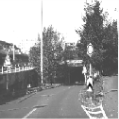
\includegraphics[width=0.32\linewidth]{figures/implementace/weights_1.png}}
    \tmpframe{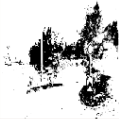
\includegraphics[width=0.32\linewidth]{figures/implementace/weights_3.png}}
    \tmpframe{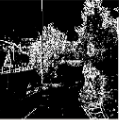
\includegraphics[width=0.32\linewidth]{figures/implementace/weights_2.png}}
    \caption{Vizualizace třech filtrů z jedné z konvolučních vrstev modelu.}
    \label{fig:weightsVis}
\end{figure}

V~průběhu trénování neuronová síť za pomoci knihovny \texttt{OpenCV} (pouze při \texttt{OPENCV=1}) vizualizuje hodnoty ztrátové funkce a~mAP na trénovací sadě, jak lze vidět na obrázku \ref{fig:chart}. Při trénování na sdíleném clusteru ovšem není možné využít GUI pro zobrazení, a~proto \emph{darknet} poskytuje možnost streamování výsledků pomocí \texttt{mjpeg} serveru na určitém portu při zadání přepínače \texttt{-mjpeg\_port <port>}. Přístup k~výsledkům je potom možný pomocí prohlížeče \url{http://<ip-address>:<port>}.

\begin{figure}[H]
    \centering
    \tmpframe{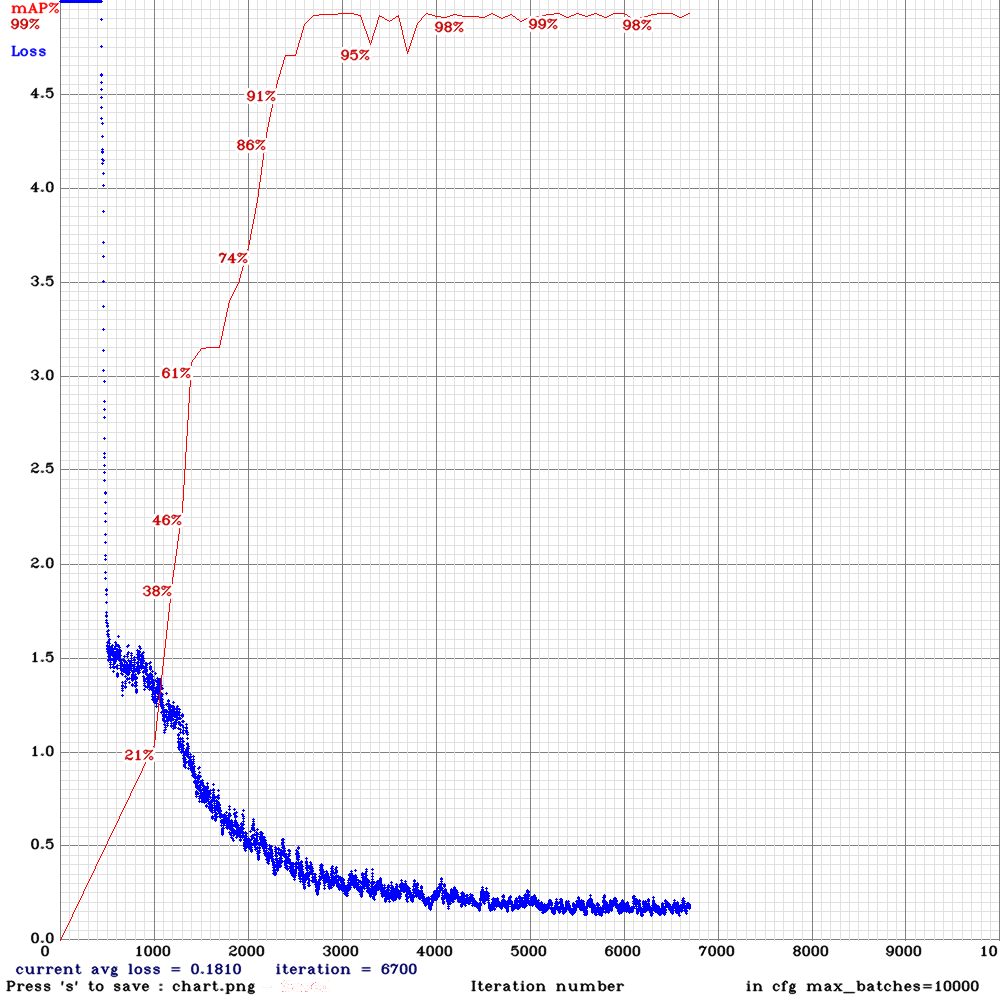
\includegraphics[width=0.8\linewidth]{figures/implementace/chart.png}}
    \caption{Výstupní obrázek \texttt{chart.png} vizualizující stav trénování neuronové sítě s~počtem iterací na ose \emph{x} a~hodnotou ztrátové funkce na ose \emph{y}. Zvyšující se červená křivka reprezentuje hodnotu mAP na validační datové sadě a~modré vzorky hodnotu ztrátové funkce při určité iteraci.}
    \label{fig:chart}
\end{figure}

Tyto hodnoty byly získány při trénování na syntetické datové sadě skládající se ze třech tříd, každá po 1000 trénovacích snímcích. Jak lze v~grafu vidět, od 6000 iterací se mAP již nezvyšuje a hodnota ztrátové funkce se zde ustálila. Ideální hodnota pro zastavení trénování je podle autorů dosažení počtu iterací 2000-krát počet tříd. To je v~tomto případě třech tříd přesně 6000 iterací. Poté začne u~modelu docházet k~jevu zvanému přetrénování, což způsobuje že model dokáže správně detekovat pouze objekty z~trénovací datové sady.

\section{Experimenty}
Poté co bylo dosaženo dobré úspěšnosti a~nedařilo se ji zvýšit za pomoci standardních metod, nastal čas provést řadu experimentů, které by mohly zajistit lepší parametry výsledného modelu.

\subsubsection*{Smíchání reálné se syntetickou datovou sadou}
Při trénování pouze na syntetické datové sadě se může konvoluční síť naučit vlastnosti vyskytující se pouze u~syntetických snímků a~nedokázat poté správně generalizovat na reálných snímcích. Proto bylo provedeno několik pokusů s~přimícháním malého počtu reálných snímku k~syntetické datové sadě. Tato malá sada reálných snímků by měla \uv{usměrňovat} trénování správným směrem a~výsledný model by poté měl dosáhnout lepší úspěšnosti na reálných snímcích. Při přidání cca. $30$ reálných snímků k~$1000$ syntetickým snímkům na třídu došlo ke zvýšení mAP o~$2\,\%$.

\subsubsection*{Hard negative mining}
\emph{Hard negative mining} je technika postupného doplňování trénovací datové sady snímky, ve kterých bylo chybně interpretováno pozadí jako některý z~detekovaných objektů.
YOLO je trénováno na plných snímcích, kde detekované objekty tvoří velmi malou část z~celého snímku a~zbytek snímku se dá tedy považovat za tzv. negativní datovou sadu, proto se může doplňující negativní datová sada zdát nadbytečná.
Po provedení několika testů se ukázalo, že ačkoli došlo ke snížení počtu falešně pozitivních detekcí, což bylo cílem, snížil se i~počet správných detekcí a~úspěšnost klesla o~$3.5\,\%$ mAP z~důvodů přetrénování.

\subsubsection*{Binární model}
Model XNOR-net pracuje jak se vstupem, tak s~vahami ve formě binárních čísel. Tento model se používá pro zvýšení rychlosti na CPU a~snížení výpočetních nároků, například pro použití v~přenosných zařízeních s~omezenými zdroji. Při testování s~uvedeným modelem došlo k~poklesu mAP o~více než $20\,\%$ oproti běžnému modelu pracujícími s~reálnými čísly a~nevýraznému zvýšení rychlosti detekce.

\subsubsection*{Přidání dalších vrstev do architektury}
V~modelu Tiny YOLOv3 se vyskytují dvě vrstvy \texttt{[yolo]} s~kotvami. Protože značky mohou nabývat různých velikostí, pokusem bylo přidání třetí takovéto vrstvy s~\texttt{mask = 6,7,8} (používající největší \emph{kotvy}) do modelu Tiny. Výsledkem byla úspěšnost obdobná modelu se dvěma vrstvami. Důvodem pravděpodobně bylo, že se v~Belgické datové sadě nevyskytuje mnoho velkých značek, které by tato vrstva detekovala.

\subsubsection*{Přepočítání kotev}
\emph{Recalculate anchors}, tedy přepočítání \uv{kotev}, slouží k~výpočtu nových hodnot tak, aby co nejlépe odpovídaly velikosti vstupních snímků. Tato technika má zvýšit průměrné \emph{IoU}, tzn. zajistit lepší úspěšnost detekce. Při přepočítání kotev na velikost vstupních snímků došlo ke zlepšení o~$0.5\,\%$ mAP.

\subsubsection*{Počáteční hodnoty modelu}
Autoři systému poskytují několik před-trénovaných vah pro různé modely. Tyto váhy byly před-trénovány na datové sadě \emph{ImageNet} a~protože konvoluční síť musí detekci hran a~tvarů umět, je lepší využít již před-trénované hodnoty. Při použití před-trénovaných vah dosáhl výsledný model o~cca. $2\,\%$ lepší mAP a~při trénování potřeboval o~2000 iterací méně, než při trénování modelu od \uv{nuly}. Z~tohoto důvodu byly při každém dalším trénování použity před-trénované váhy.


%%%%%%%%%%%%%%%%%%%%%%%%%%%%%%%%%%%%%%%%%%%%%%%%%%%%%%%%%%%%%%%%%%%%%%%%%%%%%%%%%%%%%%%%%%%


\section{Podpůrné prostředky pro trénování a~vyhodnocení}
\label{podpurneSkripty}
Konvoluční neuronová síť YOLO pracuje s~obrovským množstvím snímků doplněných o~anotace v~samostatných textových souborech, což vyžaduje jejich automatické zpracování. Stejně tak výstupem této sítě je nesčetné množství souborů s~predikcemi v~jistých formátech, které je taktéž třeba automaticky zpracovat. Z~těchto důvodů bylo vytvořeno několik skriptů pro automatické zpracování a~stejně tak použito několik již existujících. V~této podkapitole budou zmíněny nejdůležitější z~nich.

\subsection*{Trénování}
Anotace datových sad jsou běžně udávány v~různých formátech. YOLO striktně vyžaduje jistý formát, do kterého bylo potřeba tyto anotace převést. Formát anotace vyžadovaných systémem YOLO je následující:
$$\texttt{<class> <x> <y> <width> <height>}$$
Hodnota \emph{class} je celé číslo, které spadá do intervalu $\langle0,classes-1\rangle$. Parametry \emph{x}, \emph{y}, \emph{width} a~\emph{height} udávají relativní souřadnice (střed) a~proporce daného objektu vůči výšce a~šířce celého snímku. Náleží tedy do intervalu $\langle0,1\rangle$. Do tohoto formátu bylo potřeba převést anotace všech použitých datových sad (GTSD, BTSD a RTSD).

\subsection*{Vyhodnocení}
Pro predikované boxy je formát podobný, pouze je doplněn o~jistotu (confidence), s~jakou je objekt predikován a~souřadnice i~proporce objektu jsou celá čísla:
$$\texttt{<class> <confidence> <x> <y> <width> <height>}$$
Jistota spadá do intervalu $(0,1\rangle$. Pro následné vyhodnocení těchto výstupních souborů s~predikcemi vůči souborům s~\emph{ground-truth} byly v~práci využity dva repozitáře, mAP\footnotemark
\footnotetext{\url{https://github.com/Cartucho/mAP}}
a~Object-Detection-Metrics\footnotemark, implementující výpočet \emph{precission-recall} křivek, AP jednotlivých tříd a~výsledného mAP. Oba tyto repozitáře počítají s~IoU alespoň $0.5$ (tzn. aby byla predikce považována za správnou, musí se predikovaný box překrývat s~\emph{ground-truth} alespoň z~půlky, jinak je považována za falešnou), jenž je často používanou hodnotou IoU při vyhodnocení úspěšnosti detektorů.

\footnotetext{\url{https://github.com/rafaelpadilla/Object-Detection-Metrics}}